%======================================================================
% Knowledge Distillation & Quantization Toolkit -- IEEE Style Report
%======================================================================
\documentclass[conference]{IEEEtran}

%----------- Packages -------------------------------------------------
\usepackage{graphicx}
\usepackage{amsmath}
\usepackage{amssymb}
\usepackage{booktabs}
\usepackage{hyperref}
\usepackage{tikz}
\usetikzlibrary{arrows.meta, positioning, fit}
\usepackage{listings}
\usepackage{enumitem}

%----------- Metadata -------------------------------------------------
\title{Zynthe: An Enterprise Knowledge Distillation and Quantization Toolkit}

\author{\IEEEauthorblockN{Lakshin Subramanian\IEEEauthorrefmark{1}, GitHub Copilot\IEEEauthorrefmark{2}}
\IEEEauthorblockA{\IEEEauthorrefmark{1}Zynthe Research Labs, Bengaluru, India\\
Email: lakshin@zynthi.ai\\
\IEEEauthorrefmark{2}AI Programming Assistant, GitHub}}

\begin{document}
\maketitle

%----------- Abstract -------------------------------------------------
\begin{abstract}
Knowledge distillation and post-training quantization are indispensable for deploying large language models on resource-constrained hardware. This paper presents the Zynthe Knowledge Distillation and Quantization Toolkit, an enterprise-ready framework that combines modular configuration management, multi-stage distillation pipelines, quantization utilities, and evaluation/reporting suites. We describe the repository structure, workflow automation, and extensibility hooks that enable practitioners to prototype, evaluate, and productize distilled models rapidly. Case studies on IMDB sentiment analysis demonstrate how the toolkit streamlines teacher--student knowledge transfer with reproducible experiment tracking.
\end{abstract}

%----------- Keywords -------------------------------------------------
\begin{IEEEkeywords}
Knowledge distillation, quantization, model compression, large language models, enterprise AI, evaluation pipelines.
\end{IEEEkeywords}

%----------- Introduction ---------------------------------------------
\section{Introduction}
Large language models deliver state-of-the-art accuracy but often exceed the memory, latency, and energy budgets of production deployments. Knowledge distillation \cite{hinton2015distilling, buciluua2006model} compresses a high-capacity \emph{teacher} into a smaller \emph{student} network by matching logits, features, or attention distributions. Complementary post-training quantization \cite{jacob2018quantization, nagel2021whitepaper} further reduces memory footprint while preserving accuracy. Although several open-source projects implement isolated components, enterprises still require an integrated, configurable workflow that handles data preparation, experiment tracking, distillation orchestration, and quantized export.

The Zynthe Knowledge Distillation and Quantization Toolkit addresses this gap with a modular codebase that standardizes configuration, automates experiment bookkeeping, and exposes extensible APIs for custom distillers, quantizers, and evaluation tasks. This paper dissects the repository, details the core workflow, and documents the architectural patterns that make the toolkit production-ready.

%----------- Repository Overview --------------------------------------
\section{Repository Overview}
Figure~\ref{fig:architecture} illustrates the high-level architecture, while Table~\ref{tab:directories} summarizes key directories. The toolkit is organised into cohesive packages for configuration, distillation, quantization, evaluation, and deployment.

\begin{table}[!t]
    \caption{Top-Level Repository Structure}
    \label{tab:directories}
    \centering
    \begin{tabular}{ll}
        \toprule
        \textbf{Path} & \textbf{Description} \\ \midrule
        \texttt{app/} & Typer CLI for distillation/quantization commands. \\
        \texttt{configs/} & YAML presets for experiments and devices. \\
        \texttt{core/} & Library modules: config, distillers, models, quant. \\
        \texttt{data/} & JSONL datasets, preprocessing, augmentation. \\
        \texttt{docs/} & Design notes, playbooks, academic reports. \\
        \texttt{evaluation/} & Metrics, benchmarks, reporting, visualization. \\
        \texttt{examples/} & Runnable scripts and notebooks. \\
        \texttt{experiments/} & Timestamped outputs (logs, checkpoints). \\
        \texttt{training/} & Trainer, optimizer, scheduler implementations. \\
        \texttt{test/} & Automated smoke/regression tests. \\
        \bottomrule
    \end{tabular}
\end{table}

\begin{figure}[!t]
    \centering
    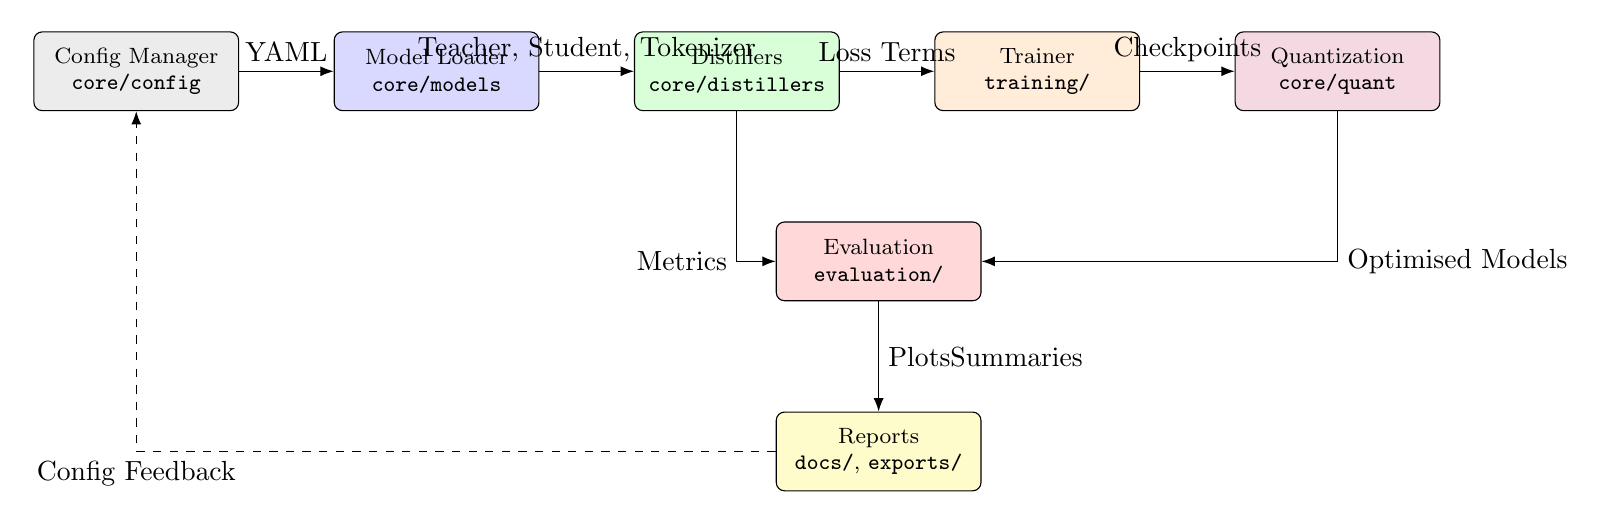
\begin{tikzpicture}[node distance=0.8cm and 1.2cm, >=Latex]
        \tikzstyle{block}=[rectangle, draw, rounded corners=3pt, align=center, minimum width=2.6cm, minimum height=1.0cm, font=\footnotesize]
        \node[block, fill=gray!15] (config) {Config Manager\\\texttt{core/config}};
        \node[block, fill=blue!15, right=of config] (models) {Model Loader \\ \texttt{core/models}};
        \node[block, fill=green!15, right=of models] (distill) {Distillers \\ \texttt{core/distillers}};
        \node[block, fill=orange!15, right=of distill] (train) {Trainer \\ \texttt{training/}};
        \node[block, fill=purple!15, right=of train] (quant) {Quantization\\\texttt{core/quant}};
        \node[block, fill=red!15, below=1.4cm of distill, xshift=1.8cm] (eval) {Evaluation \\ \texttt{evaluation/}};
        \node[block, fill=yellow!20, below=1.4cm of eval] (reports) {Reports \\ \texttt{docs/}, \texttt{exports/}};

        \draw[->] (config) -- node[above]{YAML} (models);
        \draw[->] (models) -- node[above]{Teacher, Student, Tokenizer} (distill);
        \draw[->] (distill) -- node[above]{Loss Terms} (train);
        \draw[->] (train) -- node[above]{Checkpoints} (quant);
        \draw[->] (distill) |- node[left]{Metrics} (eval);
        \draw[->] (quant) |- node[right]{Optimised Models} (eval);
        \draw[->] (eval) -- node[right]{Plots \\ Summaries} (reports);
        \draw[->, dashed] (reports) -| node[below]{Config Feedback} (config);
    \end{tikzpicture}
    \caption{Toolkit workflow: configuration drives model instantiation, distillation, training, quantization, evaluation, and reporting.}
    \label{fig:architecture}
\end{figure}

%----------- Workflow -------------------------------------------------
\section{Workflow}
The end-to-end workflow is orchestrated by the CLI (\texttt{app/main.py}) or automation scripts under \texttt{examples/}. Users customise YAML configuration files that specify teacher/student identifiers, training hyperparameters, datasets, and quantization modes. The \texttt{ConfigManager} resolves device preferences (CUDA, MPS, CPU), merges overrides, and materialises an experiment directory.

The \texttt{model\_loader} module retrieves Hugging Face models and tokenizers, wrapping the student in an enterprise \texttt{ModelWrapper} that standardises saving, quantization, and logging. Distillation strategies---such as Hinton KD, attention transfer, feature regression, and similarity matching---are composed via \texttt{MultiStageDistiller}. Each distiller inherits from \texttt{BaseDistiller}, implementing custom loss computations and hooks.

Training is handled by \texttt{training/trainer.py}, which incorporates gradient accumulation, early stopping, and mixed-precision toggles. Post-training quantization is optional and occurs through \texttt{core/quant/ptq.py}, with extensibility for quantization-aware training (QAT). Outputs are benchmarked with \texttt{evaluation/evaluator.py} and summarised using \texttt{report.py}, yielding Markdown/HTML reports under \texttt{experiments/}.

%----------- Implementation Details ----------------------------------
\section{Implementation Details}
\subsection{Configuration Layer}
The configuration manager enforces minimal schema requirements (e.g., training hyperparameters, teacher/student model names) and records Git metadata for reproducibility. Seed management ensures deterministic experimentation.

\subsection{Distillation Strategies}
\begin{itemize}[leftmargin=*, noitemsep]
    \item \textbf{Hinton KD}: Minimises Kullback--Leibler divergence between softened teacher and student logits at temperature $T$ \cite{hinton2015distilling}.
    \item \textbf{Attention Transfer}: Aligns attention maps derived from intermediate activations \cite{zagoruyko2017paying}.
    \item \textbf{Feature Regression}: Registers hooks on specified layers to regress student features toward teacher representations.
    \item \textbf{Similarity Transfer}: Encourages cosine similarity alignment for dense representations.
\end{itemize}

\subsection{Quantization Pipeline}
Dynamic post-training quantization leverages PyTorch backends (QNNPACK) with fallbacks to float16 when hardware backends are unavailable \cite{jacob2018quantization}. Future work includes integrating calibration datasets and QAT runners.

\subsection{Evaluation and Reporting}
The evaluation suite computes accuracy, F1, precision, recall, ROC-AUC, and confusion matrices using scikit-learn primitives. Reports combine numeric tables with heatmaps and ROC curves to provide decision-makers an actionable overview. Integration scripts in \texttt{test/} validate that minimal distillation and quantization flows execute end-to-end, supporting continuous integration.

%----------- Case Study ------------------------------------------------
\section{Case Study: IMDB Sentiment Compression}
The repository ships with IMDB sentiment datasets (train/validation JSONL) prepared via \texttt{data/preprocess.py}. A typical experiment distils a \texttt{distilbert-base-uncased} teacher into a compact student with minimal epochs (e.g., three) and batch sizes tuned for Apple M-series GPUs. Experiment directories capture checkpoints, resolved configurations, TensorBoard logs, and generated reports, enabling auditors to reproduce results.

%----------- Extensibility --------------------------------------------
\section{Extensibility and Roadmap}
\subsection{Enterprise Features}
Planned enhancements include CI/CD pipelines, schema validation with Pydantic, and experiment tracking integration (MLflow, Weights \\ Biases). Security-conscious deployments can layer audit logging, access control, and compliance checks.

\subsection{LLM/Agent Integration}
Future releases will expose hooks for agentic orchestration (auto-selecting distillation strategies, dynamic hyperparameter tuning) and conversational interfaces for monitoring experiments. The modular design of \texttt{MultiStageDistiller} and CLI plugs simplifies such extensions.

%----------- Conclusion ------------------------------------------------
\section{Conclusion}
Zynthe's Knowledge Distillation and Quantization Toolkit consolidates best practices in model compression within an enterprise-grade framework. By unifying configuration, distillation, quantization, and evaluation tooling, the repository accelerates the path from research to production and lays the groundwork for agent-driven optimisation.

%----------- Acknowledgements -----------------------------------------
\section*{Acknowledgements}
We thank the Zynthe research engineers and the open-source community for contributions to the PyTorch and Hugging Face ecosystems that underpin this toolkit.

%----------- References ------------------------------------------------
\begin{thebibliography}{99}
\bibitem{hinton2015distilling} G.~Hinton, O.~Vinyals, and J.~Dean, ``Distilling the knowledge in a neural network,'' in \emph{Proc. NIPS Deep Learning and Representation Learning Workshop}, 2015.

\bibitem{buciluua2006model} C.~Bucilu\u{a}, R.~Caruana, and A.~Niculescu-Mizil, ``Model compression,'' in \emph{Proc. 12th ACM SIGKDD Int. Conf.}, 2006, pp. 535--541.

\bibitem{jacob2018quantization} B.~Jacob \emph{et al.}, ``Quantization and training of neural networks for efficient integer-arithmetic-only inference,'' in \emph{Proc. IEEE CVPR}, 2018, pp. 2704--2713.

\bibitem{nagel2021whitepaper} M.~Nagel, M.~Amjad, and T.~Blankevoort, ``A white paper on neural network quantization,'' \emph{arXiv preprint arXiv:2106.08295}, 2021.

\bibitem{zagoruyko2017paying} S.~Zagoruyko and N.~Komodakis, ``Paying more attention to attention: Improving the performance of convolutional neural networks via attention transfer,'' in \emph{Proc. ICLR}, 2017.
\end{thebibliography}

\end{document}
